\documentclass[10pt, letterpaper]{article}

% Imports
\usepackage{xurl}
\usepackage{graphicx}
\usepackage{helvet}
\usepackage{fancyhdr}
\usepackage{biblatex}
\usepackage{hyperref}
\usepackage{listings}
\usepackage{xcolor}
\usepackage{float}
\usepackage[spanish]{babel}

% Settings
\pagestyle{fancy}
\addbibresource{bibliography.bib}
\fancyhead[L]{}
\hypersetup{urlcolor=yellow}
\graphicspath{ {./images/} }

% Renew commands
\renewcommand{\familydefault}{\sfdefault}
\renewcommand{\baselinestretch}{1.5}
\renewcommand{\contentsname}{Contenido}

% Create variables
\newcommand{\hmwTitle}{TRABAJO FINAL}
\newcommand{\hmwClass}{CLOUD COMPUTING E INFRAESTRUCTURA PARA BIG DATA}
\newcommand{\hmwAuthorFirst}{Bravo Peña Darlyn}
\newcommand{\hmwAuthorSecond}{Torrejón Méndez Joel Gabriel}
\newcommand{\hmwAuthorThird}{Valle Tamayo Brandon Jason}

% Setup code style
\definecolor{codegreen}{rgb}{0,0.6,0}
\definecolor{codegray}{rgb}{0.5,0.5,0.5}
\definecolor{codepurple}{rgb}{0.58,0,0.82}
\definecolor{backcolour}{rgb}{0.95,0.95,0.92}

\lstdefinestyle{mystyle}{
    backgroundcolor=\color{backcolour},   
    commentstyle=\color{codegreen},
    keywordstyle=\color{magenta},
    numberstyle=\tiny\color{codegray},
    stringstyle=\color{codepurple},
    basicstyle=\ttfamily\footnotesize,
    breakatwhitespace=false,         
    breaklines=true,                 
    captionpos=b,                    
    keepspaces=true,                 
    numbers=left,                    
    numbersep=5pt,                  
    showspaces=false,                
    showstringspaces=false,
    showtabs=false,                  
    tabsize=2
}

\lstset{style=mystyle}

% Setup title
\title{\vspace{1in}\textmd{\textbf{\hmwTitle}}\\\vspace{0.5in}\textmd{\hmwClass}\\\vspace{2.5in}}
\date{}
\author{\textnormal{\hmwAuthorFirst}\\\textnormal{\hmwAuthorSecond}\\\textnormal{\hmwAuthorThird}}

% Init document
\begin{document}
\maketitle
\thispagestyle{empty}

% Table of contents
\newpage
\thispagestyle{plain}
\tableofcontents
\listoffigures

% Homework parts
\newpage
\section{Base de Datos}
\subsection{Recopilación}
Para este proyecto nosotros decidimos utilizar un dataset público
\textbf{IBM HR Analytics Employee Attrition and Performance} \cite{ibm-hr},
este data set se enfoca en la rotación de empleados en una empresa, analizando
varios aspectos de los empleados, como su salario, horas de trabajo, etc.

\subsubsection{Atributos}
El dataset cuenta con 35 atributos, los cuales son:
\begin{itemize}
    \item \textbf{Age:} Edad del empleado.
    \item \textbf{Attrition:} Si el empleado ha dejado la empresa o no.
    \item \textbf{BusinessTravel:} Frecuencia de viajes de negocios.
    \item \textbf{DailyRate:} Salario diario.
    \item \textbf{Department:} Departamento en el que trabaja el empleado.
    \item \textbf{DistanceFromHome:} Distancia de la casa al trabajo.
    \item \textbf{Education:} Nivel de educación.
    \item \textbf{EducationField:} Campo de estudio.
    \item \textbf{EmployeeCount:} Cantidad de empleados.
    \item \textbf{EmployeeNumber:} Número de empleado.
    \item \textbf{EnvironmentSatisfaction:} Satisfacción con el ambiente de trabajo.
    \item \textbf{Gender:} Género.
    \item \textbf{HourlyRate:} Salario por hora.
    \item \textbf{JobInvolvement:} Nivel de involucramiento en el trabajo.
    \item \textbf{JobLevel:} Nivel de trabajo.
    \item \textbf{JobRole:} Rol en la empresa.
    \item \textbf{JobSatisfaction:} Satisfacción con el trabajo.
    \item \textbf{MaritalStatus:} Estado civil.
    \item \textbf{MonthlyIncome:} Ingreso mensual.
    \item \textbf{MonthlyRate:} Ingreso mensual.
    \item \textbf{NumCompaniesWorked:} Número de empresas en las que ha trabajado.
    \item \textbf{Over18:} Si es mayor de 18 años.
    \item \textbf{OverTime:} Si trabaja horas extras.
    \item \textbf{PercentSalaryHike:} Porcentaje de aumento salarial.
    \item \textbf{PerformanceRating:} Calificación de desempeño.
    \item \textbf{RelationshipSatisfaction:} Satisfacción con las relaciones.
    \item \textbf{StandardHours:} Horas estándar.
    \item \textbf{StockOptionLevel:} Nivel de opciones de acciones.
    \item \textbf{TotalWorkingYears:} Años trabajados.
    \item \textbf{TrainingTimesLastYear:} Horas de entrenamiento el año pasado.
    \item \textbf{WorkLifeBalance:} Balance entre trabajo y vida personal.
    \item \textbf{YearsAtCompany:} Años en la empresa.
    \item \textbf{YearsInCurrentRole:} Años en el rol actual.
    \item \textbf{YearsSinceLastPromotion:} Años desde la última promoción.
    \item \textbf{YearsWithCurrManager:} Años con el actual jefe.
\end{itemize}


\subsection{Variables a analizar}
De todas las variables descritas anteriormente, nosotros decidimos analizar las
siguientes 9 variables:
\begin{itemize}
    \item \textbf{Age:} Edad del empleado.
    \item \textbf{MonthlyIncome:} Ingreso mensual.
    \item \textbf{NumCompaniesWorked:} Número de empresas en las que ha trabajado.
    \item \textbf{TotalWorkingYears:} Años trabajados.
    \item \textbf{YearsAtCompany:} Años en la empresa.
    \item \textbf{YearsInCurrentRole:} Años en el rol actual.
    \item \textbf{YearsSinceLastPromotion:} Años desde la última promoción.
    \item \textbf{YearsWithCurrManager:} Años con el actual jefe.
    \item \textbf{JobLevel:} Nivel de trabajo.
\end{itemize}
\newpage
\section{Preparación de datos}
\subsection{Enunciado}
Estandarización: Antes de aplicar PCA, asegúrate de estandarizar las variables cuantitativas para que tengan media cero y desviación estándar uno. Esto es importante, ya que PCA es sensible a la escala de los datos. Nota: Sklearn utiliza la matriz de covarianza y esa es la razón por la que hay que estandarizar previamente. 

Matriz de Correlación: Visualizar la matriz de correlación de las variables originales antes de aplicar PCA. Como regla general:
Un rango óptimo de correlación entre variables se sitúa entre ±0.5 y ±0.9. Las correlaciones más bajas indican que las variables no están relacionadas, lo que podría implicar que PCA no reducirá significativamente la dimensionalidad. Si la correlación entre muchas variables es cercana a cero, PCA puede no ser tan efectivo. Idealmente, deberías observar varias correlaciones moderadas a fuertes entre las variables.

\subsection{Estandarización de datos}
Tomando en cuenta las variables que se utilizarán, esto nos muestra la transformación utilizando Sklearn para el escalado de la misma.

\begin{table}[H]
\centering
\begin{tabular}{|l|r|}
\hline
\textbf{Variable} & \textbf{Media} \\ \hline
Age                       & -3.504377e-17 \\ \hline
DailyRate                  &  5.075305e-17 \\ \hline
HourlyRate                 &  1.691768e-16 \\ \hline
MonthlyIncome              & -4.471102e-17 \\ \hline
MonthlyRate                &  3.021015e-17 \\ \hline
NumCompaniesWorked         &  1.450087e-17 \\ \hline
TotalWorkingYears          & -1.208406e-18 \\ \hline
YearsAtCompany             & -3.021015e-17 \\ \hline
YearsInCurrentRole         &  9.063045e-17 \\ \hline
YearsSinceLastPromotion    &  1.208406e-18 \\ \hline
\end{tabular}
\caption{Media de cada variable estandarizada}
\end{table}

\textbf{Observación:}
Podemos evidenciar en el siguiente cuadro que la media está 
cerca de 0 (por ejemplo, entre -1e-17 y 1e-18).

\begin{table}[H]
\centering
\begin{tabular}{|l|r|}
\hline
\textbf{Variable} & \textbf{Desviación Estándar} \\ \hline
Age                        & 1.00034 \\ \hline
DailyRate                  & 1.00034 \\ \hline
HourlyRate                 & 1.00034 \\ \hline
MonthlyIncome              & 1.00034 \\ \hline
MonthlyRate                & 1.00034 \\ \hline
NumCompaniesWorked         & 1.00034 \\ \hline
TotalWorkingYears          & 1.00034 \\ \hline
YearsAtCompany             & 1.00034 \\ \hline
YearsInCurrentRole         & 1.00034 \\ \hline
YearsSinceLastPromotion    & 1.00034 \\ \hline
\end{tabular}
\caption{Desviación estándar de cada variable estandarizada}
\end{table}

\subsection{Matriz de correlación}
Utilizando los datos estandarizados, se procede a calcular la matriz de correlación.

\begin{figure}[h!]
    \centering
    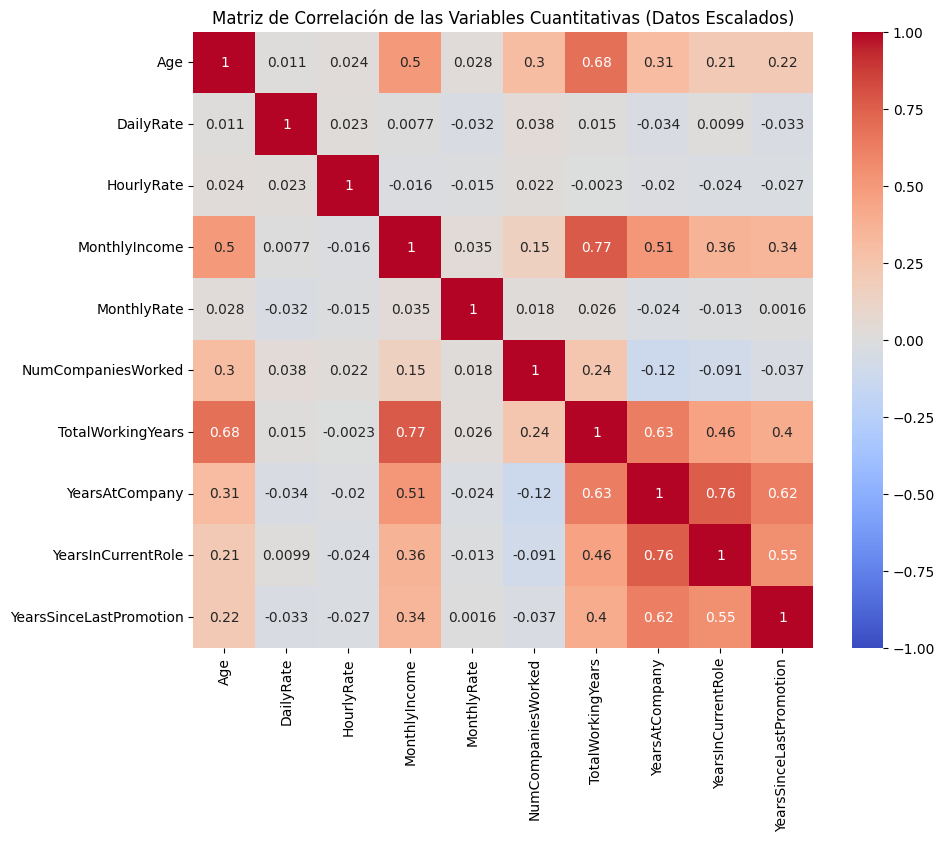
\includegraphics[width=1\textwidth]{images/matriz-de-correlacion.png}
    \caption{Matriz de correlación de las variables cuantitativas}
    \label{fig:matriz_correlacion}
\end{figure}

Podemos observar que la matriz de correlación es una matriz simétrica, 
con valores en la diagonal principal iguales a 1, aunque vemos que las variables
DailyRate, HourlyRate, MonthlyRate y NumCompaniesWorked tienen una correlación cercana a 0
lo que indica no hay una relación lineal fuerte entre esa una variable y otra en la matriz.

\newpage
\thispagestyle{plain}
\printbibliography[heading=bibintoc]

\end{document}